
\newcommand {\matr}[2]{\left[\begin{array}{#1}#2\end{array}\right]}
\newcommand{\E}{\mathbb{E}}
\newcommand{\tr}{\mathrm{tr}}
\newcommand{\x}{{\mathbf{x}}}
\renewcommand{\u}{{\mathbf{u}}}
\newcommand{\w}{{\mathbf{w}}}
\renewcommand{\r}{{\mathbf{r}}}

\definecolor{wheat}{rgb}{0.96,0.87,0.70}
\definecolor{lightblue}{rgb}{0.8,0.8,1}
\definecolor{lightred}{rgb}{1,0.8,0.8}
\definecolor{lightgreen}{rgb}{0.8,1,0.8}

% \newcommand\argmax{\mathop{\rm arg\,max}}
% \newcommand\argmin{\mathop{\rm arg\,min}}
% \newcommand {\defn} {\triangleq}
% \newcommand \Reals {\ensuremath{\mathbb{R}}}
% \newcommand \E {\mathop{\mbox{\ensuremath{\mathbb{E}}}}\nolimits}
% \newcommand \V {\mathop{\mbox{\ensuremath{\mathbb{V}}}}\nolimits}
% \renewcommand \Pr {\mathop{\mbox{\ensuremath{\mathbb{P}}}}\nolimits}
% %\newtheorem{lemma}{Lemma}
% %% macros for symbols
\newcommand \pol {\pi}
\newcommand \Pol {\Pi}
% \newcommand \bel {\beta}
\newcommand \mdp {\mu}
\newcommand \MDP {\mathcal{M}}
\newcommand \return {R}
\newcommand \utility {U}
\newcommand \GP {\mathcal{GP}}
\newcommand \param {\theta} %% unknown parameter
\newcommand \Params {\Theta} %% unknown parameter



\newcommand \disc {\gamma}
\newcommand \MDPs {\mathcal{M}} %% The MDP
\newcommand \Pols {\Pi} %% The policy
\newcommand \VC[3] {V_{#1,#2}^{#3}}
\newcommand \VS[2] {V_{#1,#2}^{*}}
\newcommand \CS {\mathcal{S}} %% The state space
\newcommand \CA {\mathcal{A}} %% The action space
\newcommand \CV {\mathcal{V}} %% The value function estimate
\newcommand \trans {\mathcal{T}} %% The transition kernel
\newcommand \rew {\rho} %% The reward function\newcommand \disc {\gamma} %% discount factor
\newcommand \abel {\hat{\xi}} %% approximate belief
\newcommand \mbel {\psi} %% belief about MDPs 

\newcommand \p {\partial}

\newcommand \Bellman {\mathscr{L}}
\newcommand \PBellman {\mathscr{P}}
\newcommand \util {U}
\newcommand \val {\vectorsym{v}}
\newcommand \Vals {\mathcal{V}}
\newcommand \discount {\gamma}
\newcommand \horizon {T}

%% Commands

% \DeclareMathOperator{\st}{s.t.\,}
% \DeclareMathOperator{\trace}{tr}

\newcommand \onenorm[1]{\left\|#1\right\|_1}
\newcommand \pnorm[2]{\left\|#1\right\|_{#2}}
\newcommand \inftynorm[1]{\left\right\|#1\|_\infty}
\newcommand \norm[1]{\left\|#1\right\|}


\newcommand \dd {\, \mathrm{d}}
\let\Pr\relax
\newcommand \Pr {\mathbb{P}}

\newcommand \cset[2] {\left\{#1 ~\middle|~ #2\right\}}
\newcommand \set[1] {\left\{#1\right\}}
\newcommand \ind[1] {\mathds{1}\left\{#1\right\}}

\newcommand \KL[2] {D\left( #1 ~\middle\|~ #2\right)}

% \DeclareMathAlphabet{\mathpzc}{OT1}{pzc}{m}{it}

\newcommand \Softmax {{\mathpzc{Softmax}}}
\newcommand \GammaDist {{\mathpzc{Gamma}}}
\newcommand \Dirichlet {{\mathpzc{Dir}}}
\newcommand \Uniform {{\mathpzc{Unif}}}
\newcommand \Bernoulli {{\mathpzc{Bern}}}
\newcommand \Binomial {{\mathpzc{Binom}}}
\newcommand \Beta {{\mathpzc{Beta}}}
\newcommand \Geometric {{\mathpzc{Geom}}}
\newcommand \Normal {{\mathpzc{N}}}
\newcommand \Multinomial {{\mathpzc{Mult}}}
\newcommand \Wishart {{\mathpzc{Wish}}}


\if 1
\newcommand \note[2][blue] {{\color{#1} \texttt{[#2]}}}
\newcommand \cor[2][red] {{\color{#1}#2}}
\newcommand \ins[2][magenta] {{\color{#1}#2}}
\newcommand \del[2][red] {{\color{#1}\sout{#2}}}
\newcommand \grm[2][green!50!black] {{\color{#1}#2}}
\else

\newcommand \ins[2][magenta] {{\color{#1}#2}}
\fi

%%% other notes
\newcommand\hecomment[1]{{\color{red}{[HE: \texttt{#1}]}}}
\newcommand\cdcomment[1]{\texttt{[CD: #1]}}
\newcommand\dbcomment[1]{{\color{magenta}{[DB: \texttt{#1}]}}}
\newcommand\ttcomment[1]{{\color{orange}{[TT: \texttt{#1}]}}}
\newenvironment{mycomments}[1]{%
	\leavevmode\color{#1}\ignorespaces%
}{%
}%


%%%%%%%%%%%%%%%%%%%%%%%%%%%%%%%%%%%%%%%%%%%%%%%%%%%%%%%%%%%%%%%%%%%%%%%%%%%%%%%%
\begin{abstract}
    For decision-problems with insufficient data, it is imperative to take into account not only what you know but also what you do not know. In this work, ways of transferring knowledge from known, existing tasks to a new setting is studied. In particular, for tasks such as autonomous driving, the optimal controller is conditional on things such as, the physical properties of the vehicle, the local and regional traffic rules and regulations and also on the specific scenario trying to be solved. Having separate controllers for every combination of these conditions is intractable. By assuming problems with similar structure, we are able to leverage knowledge attained from similar tasks to guide learning for new tasks. We introduce a maximum likelihood estimation procedure for solving Transfer Reinforcement Learning (TRL) of different types. This procedure is then evaluated over a set of autonomous driving settings, each of which constitutes an interesting scenario for autonomous driving agents to make use of external information. We prove asymptotic regret bounds for proposed method for general structured probability matrices in a specific setting of interest.
\end{abstract}
\section{Introduction}\label{sec:intro}

%%% GENERAL OVERVIEW
Sequential decision-making for autonomous driving agents has been studied under the Reinforcement Learning (RL) framework, which involves actively interacting with an environment for it to be able to improve on its performance. Disregarding the apparent difficulty in learning decision-making agents for large-scale environments, this also gives rise to another set of problems. For one, how do you guarantee safe performance during the learning process and secondly, how can you leverage external knowledge about decision-making problem. For instance, there might be information available informing us on how to act in a particular autonomous driving task, such as in an overtake scenario, that can be used to make decisions on how to act in a related task, such as a cut-in scenario, where another vehicle is changing lane onto the ego vehicle's lane.

%%% 

Motivations for transfer learning in the context of autonomous driving are multifold. For instance, learning a controller for a particular vehicle involves figuring out what decision-making behavior is optimal given the properties of the vehicle. If the vehicle is less insert, you could expect more hasty decision-making is possible, whereas for a large vehicle like a semi-trailer truck, the decision to accelerate or decelerate needs to be made way in advance of the traffic situation. Furthermore, one could expect the learned controller to be locally optimal in the region it has collected data in. However, learning a global controller that is able to handle all sorts of local traffic rules and regulations, left- and right-hand traffic and the behavior of other road users is not easy. Thus, the framework proposed in this work can alleviate concerns regarding learning optimal controllers for each separate vehicle type, scenario and geographic region by leveraging knowledge transfer and sharing data across problems.

%% add references to the classical dagger, gail, etc works that use expert policies / demonstrations
Similar topics have been studied in the context of \emph{transfer machine learning}, e.g. in imitation learning. Recently, a lot of interest has been shown for \emph{transfer reinforcement learning} in e.g. \cite{zhu2020transfer}, where RL agents are able to learn how to act in environments by transferring knowledge from experts to facilitate the learning process. Typically, this has been done by two particular methods, firstly, \emph{learning by demonstrations}, where agents are given data trajectories of demonstrations or expert policies from which they are able to bootstrap knowledge about the task. Secondly, the agent may have access to model dynamics of similar tasks, from which it could be able to extract knowledge from to guide learning in the actual environment.

These two approaches are denoted \emph{policy transfer} and \emph{model transfer}, respectively, by~\cite{zhu2020transfer}.

%%% CONTRIBUTION

\subsection{Related Work}\label{sec:related}

\hecomment{TODO: Write about the uncommented works in this related work section.}

\subsection{Contribution}
In this work, we develop methods for leveraging knowledge transfer in the context of reinforcement learning. By identifying a global model that takes into account existing information from other tasks, we can design a decision-making agent capable to handling multiple unknown scenarios at once, by using the current observed information of the task together with knowledge from similar tasks. The maximum likelihood global model parameters are identified and the optimal controller for the global model can attained through typical reinforcement learning means. The optimal global model under this formulation can change with time as more data is observed from the target task.
The framework is evaluated in both discrete MDP scenarios and a larger, more complicated autonomous driving experiment where multiple transfer learning situations for autonomous driving are considered.

\hecomment{Some illustrative TRL problem for AD, for example AD in US, Sweden and India showing different traffic scenarios. We try to build a global model.}
\ttcomment{TRL examples suggestions: trained for low speed traffic jams, transfer to a high speed highway driving. 
traffic laws in different countries. some part of the us allow turning right in an intersection when the traffic light is red. Sweden usually have slower speed limitations on the road, Asia has higher traffic density.}
%%%

%%% OUTLINE

In Section~\ref{sec:background} the necessary background details are described, such as the likelihoods used, the feature representations and the model definition.


%%%

%%% Risk-sensitive MARL

\iffalse
Risk-sensitive MARL:

\begin{itemize}
    \item RMIX: Learning Risk-Sensitive Policies for Cooperative
Reinforcement Learning Agents\url{https://arxiv.org/pdf/2102.08159.pdf}
\end{itemize}
\fi

%%%

%%%

%%% Bayesian Multi-task Reinforcement Learning (Wilson07, Lazaric10)

\iffalse
Bayesian Multi-Task RL: 

\begin{itemize}
    \item Multi-Task Reinforcement Learning: A Hierarchical Bayesian Approach \url{http://engr.case.edu/ray_soumya/papers/mtrl-hb.icml07.pdf}
    \item Bayesian Multi-Task Reinforcement Learning \url{https://icml.cc/Conferences/2010/papers/269.pdf}
    \item Bayesian Hierarchical Reinforcement Learning \url{https://proceedings.neurips.cc/paper/2012/file/642e92efb79421734881b53e1e1b18b6-Paper.pdf}
\end{itemize}
\fi

%%%

%%%

%%% Meta-Learning (whole body of work on say MAML by Abbeel/Sergie Levine

\iffalse
Meta-Learning:

\begin{itemize}
    \item Online meta-learning \url{http://proceedings.mlr.press/v97/finn19a/finn19a.pdf}
    \item Meta-Learning: A Survey \url{https://arxiv.org/pdf/1810.03548.pdf}
\end{itemize}
\fi

%%%

%%%

%%% Learning mixtures in a Bayesian way

\iffalse
Learning Bayesian mixtures:

\begin{itemize}
    \item Bayesian Classifier Combination \url{http://proceedings.mlr.press/v22/kim12/kim12.pdf}
    \item Bayesian Combination of Probabilistic Classifiers using Multivariate Normal Mixtures \url{https://www.jmlr.org/papers/volume20/18-241/18-241.pdf}
\end{itemize}
\fi

%%%

\iffalse
Federated Ensemble Model-based Reinforcement Learning \url{https://arxiv.org/pdf/2109.05549.pdf}

Federated Control with Hierarchical Multi-Agent Deep Reinforcement Learning \url{https://arxiv.org/pdf/1712.08266}
Federated learning with hierarchical clustering of
local updates to improve training on non-IID data \url{https://arxiv.org/pdf/2004.11791.pdf}
Hierarchical Federated Learning Across Heterogeneous Cellular Networks \url{https://arxiv.org/pdf/1909.02362}
Hierarchical Federated Learning through LAN-WAN Orchestration \url{https://arxiv.org/pdf/2010.11612}
Client-Edge-Cloud Hierarchical Federated Learning \url{https://arxiv.org/pdf/1905.06641}
Transfer Learning in Deep Reinforcement
Learning: A Survey-- \url{https://arxiv.org/pdf/2009.07888.pdf} 
Reinforcement Learning in Parametric MDPs
with Exponential Families \url{https://proceedings.mlr.press/v130/chowdhury21b/chowdhury21b.pdf}
Learning Robust Controllers for Linear Quadratic Systems
with Multiplicative Noise via Policy Gradient -- \url{http://www.dcsc.tudelft.nl/~mohajerin/Publications/journal/2019/stochastic_LQR.pdf}
iLQR -- \url{https://katefvision.github.io/katefSlides/RECITATIONtrajectoryoptimization_katef.pdf}
Distributed Reinforcement Learning for Decentralized Linear Quadratic Control- \url{https://arxiv.org/pdf/1912.09135.pdf}
\fi

\section{Background}\label{sec:background}

In this section, we will be introducing important concepts on which this work is based upon.

\subsection{Markov Decision Process}

In this work, we are studying sequential decision-making problems that are able to be modelled by Markov Decision Processes (MDPs)~\cite{sutton2018reinforcement}. An MDP $\mdp$ consists of the following constructs, $\mathcal{S} \in \mathbb{R}^d$, which is the state-space of the problem of dimension $d$. $\mathcal{A}(s)$ is the set of possible actions to take in state $s$. $\mathcal{R} : \mathcal{S}\times\mathcal{A}\rightarrow \mathbb{R}$ is a reward function which determines the quality of taking a particular action $a$ in state $s$. $\mathcal{T} : \mathcal{S}\times \mathcal{A} \rightarrow \Delta(\mathcal{S})$ is a transition kernel that describes how states evolve in the MDP. Finally, $\gamma$, is the discount factor chosen for the problem.

The objective of an agent acting in a MDP is to arrive at a policy $\pol : \mathcal{S} \rightarrow \Delta(\mathcal{A})$ that maximises the expected sum of future discounted rewards up until the horizon $T$. $V_\mdp^\pol(s) = \mathbb{E}\Big[\sum_{t=0}^T \gamma^t R(s_t, a_t)\Big]$.

\iffalse
\subsection{Risk-sensitive RL}

\hecomment{Might not need RSRL}
If a random variable $Z \in \mathcal{Z}$ follows a distribution $P$, a risk measure is a function $U : \mathcal{Z} \rightarrow \mathbb{R}$. In the context of RL, the quantities of interest that a risk-sensitive agent might consider is the variation in returns $Z$, where $Z(s,a) \defn \sum_{t=0}^T \gamma^t R(s_t, a_t)$. These variations occur due to the inherent stochasticity of MDP $\mdp$ and the policy $\pol$ (if stochastic) and are commonly termed as the aleatory uncertainty. Another source of uncertainty occurs when the parameters of the MDP $\mdp$ are unknown, for instance in cases where a posterior over MDPs $\xi(\mdp)$ is considered. The random variable of interest in that case is then $\mathbb{E}_\mdp^\pi[Z]$ where $\mdp$ follows the distribution $\xi$.
\fi

\subsection{Likelihoods}

For discrete MDPs, we use product over each $s, a$ pair of multinomials as likelihood, $\Pr(\mathcal{D}_t \, | \, \mdp) = \prod_{s,a}\frac{n!}{s_0!, ..., s_{|\mathcal{S}|}!}p(s' = s_0 \, | \, s=s_0, a=a_0)^{x_0}\\ \cdots p(s' = s_{|\mathcal{S}|} \, | \, s=s_0, a=a_0)^{x_{|\mathcal{S}|}}$.

For linear MDPs, we use linear models $\mathcal{N}(\bm{s}^\top\bm{\mdp}_t, \Sigma_t)$ as models. The likelihood is then a product of Gaussians, one for each $(s, a \rightarrow s') \in \mathcal{D}_t$.

Constraints on $\Sigma_t$, positive semi-definite, symmetric. IF we are even a weight vector $\bm{w}$, and the objective is to create a mean model, averaged over $\bm{w}$, $\mathbb{E}_{\bm{w}}[\mathcal{M}_s]$, when $\mathcal{M}_s$ is a set of linear-Gaussian models, then $\mdp_{\bm{w}} = \sum_{i=1}^K w_i \bm{\mdp}_i, \Sigma_{\bm{w}} = \sum_{i=1}^K w_i \Sigma_i$. $\Sigma_{\bm{w}}$ is guaranteed to be PSD as well.

\subsection{Feature Representations}

Doing model-based RL for settings with large and complicated state spaces, there might be some need for appropriate feature representations. In this work, we make use of randomised fourier features, based on the work of~\cite{ren2021free}.

\section{Transfer Reinforcement Problem Formulation}\label{sec:trl}

\begin{table*}[!t]
\centering
\caption{Examples of related TRL works}
\begin{tabular}{ |p{6cm}|p{5cm}|  }
 \hline
 \multicolumn{2}{|c|}{Classes of Transfer Reinforcement Learning problems} \\
 \hline
 Parameter space&Related work\\
 \hline
 \textsc{Type I:} Finite parameter set $\Theta$ & ref1, ref2, ref3, ref4\\
 \textsc{Type II:} Infinite, convex set $\Theta$ & ref1, ref2, ref3, ref4\\
 \textsc{Type III:} Infinite, bounded set $\Theta$ & ref1, ref2, ref3, ref4\\
 \textsc{Type IV:} Arbitrary set $\Theta$& ref1, ref2, ref3, ref4\\
 \hline
\end{tabular}
\end{table*}

Reinforcement learning for transfer learning augments the previous definition of MDPs through the consideration of \emph{source} and a \emph{target} domain. Given a set of source domains $\Theta_s = \{\theta^1, \cdots, \theta^K\} \in \Theta^K$ and a target domain $\theta_t \in \Theta$, we wish to leverage knowledge transfer from $\Theta_s \rightarrow \theta_t$. If $\theta \in \Theta_s$, we call this setting a \textsc{Type I} setting and the considered set of $\theta$ is finite. If $\theta \in \mathcal{C}(\Theta_s)$, where $\mathcal{C} : \Theta^K \times [0, 1]^K \rightarrow \Theta$ is the convex set spanned by each of the $\theta \in \Theta^K$, then we call this a setting of \textsc{Type II} with infinite and realisable plausible models. If the assumptions on $\theta$ is relaxed even more, and now $\theta \in \delta(\Theta_s)$, where $\delta(\Theta_s)$ is the set of MDPs that are $\delta$ close to $\Theta_s$, then we term this \textsc{Type III} and it is the set of infinite and non-realisable bounded plausible models. Finally, for \textsc{Type IV}, we consider arbitrary MDPs $\theta \in \Theta$.

\hecomment{TODO: explain the different settings here}
\ttcomment{introduce the TYPEs intuitive names here, the names on the subsections}

\subsection{Finite and realisable plausible models}

For the first type of Bayesian TRL the parameters of the source models $\mdp \in \mathcal{M}_s$ are known, and the target model $\mdp_t \in \mathcal{M}_s$. $\mdp_t$ is unknown, but data $\mathcal{D}_t \sim \mdp_t$ exists. This setting reduces to one of hierarchical Bayesian RL where the initial goal is to identify the posterior $\Pr(\mdp \in \mathcal{M}_s \, | \, \mathcal{D}_t)$. When this has been attained, we can obtain the optimal controller $\pol_{\textrm{Type I}}^{*}$ by maximising over policies $\pol \in \Pi$.

\begin{equation}
    \pol_{\textrm{Type I}}^{*} = \underset{\pol}{\arg \max} \, V_\mdp^\pol \Pr(\mdp \in \mathcal{M}_s \, | \, \mathcal{D}_t) 
\end{equation}

\subsection{Infinite and realisable plausible models}

In this setting we can arrive at two different solution methods, one \emph{interior point method} and one fully Bayesian method with a constrained prior over the convex set of MDPs $\mathcal{C}(\mathcal{M}_s)$.

The interior point method starts by selecting a point $\bm{p}_0 \in [0, 1]^K$ in the simplex with $\mdp \in \mathcal{M}_s$ being the vertices. A point in the simplex defines a convex combination of the known MDPs at the vertices. Iteratively, we can arrive at better and better points $\bm{p}_1, ..., \bm{p}_T$ by using the likelihood $\Pr(\mathcal{D}_t \, | \, \bm{p})$. Eventually, the procedure will converge at a point $\bm{p}_{*}$, this is the point in the simplex that represents the maximum likelihood MDP $\mdp^{*}$. Of course the constraints are linear, (transitions), however, the likelihood is not convex.

Another method would be a gradient based method used to find the maximum likelihood MDP $\Pr(\mathcal{D}_t \, | \, \mdp \in \mathcal{C}(\mathcal{M}_s))$.

\begin{equation}
    \mdp^{*} = \underset{\mdp \in \mathcal{C}(\mathcal{M}_s)}{\arg \max} \, \Pr(\mathcal{D}_t \, | \, \mdp)
\end{equation}

\begin{equation}
    \pol_{\textrm{Type III}}^{*} = \underset{\pol}{\arg \max} \, V_{\mdp^{*}}^\pol
\end{equation}

This is identical to the following,
\begin{equation}
\begin{aligned}
w^{*} = \underset{w}{\arg\min} \quad & -\Pr(\mathcal{D}_t \, | \, \mathbb{E}_w [\mathcal{M}_s])\\
\textrm{s.t.} \quad & \sum_{i=1}^K w_i = 1\\
  &\forall_w \, 0 \leq w_i \leq 1,    \\
\mdp^{*} = \quad \mathbb{E}_{w^{*}}[\mathcal{M}_s]\\
\pol^{*}_{\textrm{Type III}} = \underset{\pol}{\arg\max} \, V_{\mdp^{*}}^\pol
\end{aligned}
\end{equation}

We can also consider a prior over the convex set of MDPs $\mathcal{C}(\mathcal{M}_s)$, such as the Dirichlet prior. Thus the posterior $\Pr(\mdp \in \mathcal{C}(\mathcal{M}_s) \, | \, \mathcal{D}_t)$ only has support over the simplex spanned by $\mathcal{C}(\mathcal{M}_s)$ in model space $\mathcal{M}$. In this case, the optimal Bayesian controller could be written as the following,

\begin{equation}
  \pol_{\textrm{Type III}}^{*} = \underset{\pol}{\arg \max} \, \int_{\mathcal{C}(\mathcal{M}_s)} V_\mdp^\pol \dd \Pr(\mdp \, | \, \mathcal{D}_t).
\end{equation}

A third possible approach is a variational Bayes approach, where the goal is to identify the parameters of the posterior (Dirichlet, with multinomial likelihood). The optimisation routine would then find the parameters of this posterior.

\subsection{Infinite and non-realisable bounded plausible models}

For the type V setting we have no structural constraints on the target MDP $\mdp_t$ and it can be outside the convex set of MDPs spanned by $\mathcal{M}_s$. Typically, to make this approach possible, we can apply some kind of constraints of the differences between the target MDP $\mdp_t$ and the source MDPs $\mathcal{M}_s$. For example, $KL(\mdp_t \, || \, \frac{1}{N}\sum_{\mdp \in \mathcal{M}_s} \mdp) \leq \delta$, for discrete MDPs and e.g. the spectral radius / Eigenvalue of linear MDPs.

\paragraph{Constrained}
\begin{equation}
\begin{aligned}
\mdp^{*} = \quad &\underset{\mdp}{\arg\max} \, \Pr(\mathcal{D}_t \, | \, \mdp)\\
\textrm{s.t.} \quad & \textrm{KL}(\mdp \, || \, \mathbb{E}[\mathcal{M}_s]) \leq \delta.\\
\pol^{*}_{\textrm{Type V}} &= \underset{\pol}{\arg\max} \, V_{\mdp^{*}}^\pol
\end{aligned}
\end{equation}

\paragraph{Unconstrained}
\begin{equation}
\begin{aligned}
\mdp^{*} &= \underset{\mdp}{\arg\max} \, \Pr(\mathcal{D}_t \, | \, \mdp) - \lambda\textrm{KL}(\mdp \, || \, \mathbb{E}[\mathcal{M}_s])\\
\pol^{*}_{\textrm{Type V}} &= \underset{\pol}{\arg\max} \, V_{\mdp^{*}}^\pol
\end{aligned}
\end{equation}

Currently we use a trust region method to optimise with $|\mathcal{S}|$ linear constraints, one for each $p(s' \, | \, s, a)$ pair, and $|\mathcal{S}|^2\times |\mathcal{A}|$ bounds. We use the unconstrained method as the addition of the KL bound would introduce non-linear constraints.

\begin{equation}
\begin{aligned}
\mdp^{*} &= \underset{\mdp}{\arg\max} \, \Pr(\mathcal{D}_t \, | \, \mdp) - \lambda\textrm{KL}(\mdp \, || \, \mathbb{E}[\mathcal{M}_s])\\
\textrm{s.t.} \quad & \mathbf{A}\bm{p} = \bm{1},\\
\quad \quad & \bm{0} \leq \bm{p} \leq \bm{1}.\\
\pol^{*}_{\textrm{Type V}} &= \underset{\pol}{\arg\max} \, V_{\mdp^{*}}^\pol
\end{aligned}
\end{equation}

\subsection{Infinite and arbitrary plausible models}

\section{Maximum Likelihood Estimation of MDPs in Transfer Reinforcement Learning}\label{sec:MLE}

\subsection{Discrete MDPs}
\paragraph{Incorporating the Structure.}
In this section we study general structured probability matrices with \begin{align}
    &\sum_{s'} p(s' \, | \, s, a) = 1,\\
    \forall_{(s, s', a) \in \mathcal{S}^2\times\mathcal{A}} \, &0 \leq p(s' \, | \, s, a) \leq 1.
\end{align}

The likelihood $\mathcal{L}(\mathcal{D}, \theta)$ is a product over all the likelihoods for the individual transitions $p(s' \, | \, s, a)$ and in this case, a product of \emph{multinomials}.

\begin{equation}
    \mathcal{L}(\mathcal{D}, \theta) = \prod_{s, a} \frac{n!}{x_1! \cdots x_{|\mathcal{S}|}!}\theta_1^{x_1} \cdots \theta_{|\mathcal{S}|}^{x_{|\mathcal{S}|}} 
\end{equation}

As the parameter $\theta$ that maximises this likelihood will also maximise the log likelihood $\log \mathcal{L}(\mathcal{D}, \theta)$, we will choose to write it in this form. The log-likelihood of a multinomial random variable can be written as,

\begin{equation}
    \log \mathcal{L}(x_i, n \, | \, \theta) = \log(C) + \sum_{i=1}^k x_i \log \theta_i.
\end{equation}

The product over $|\mathcal{S}|\times|\mathcal{A}|$ of pairs of these multinomials is thus,

\begin{align}
    \log \mathcal{L}(\mathcal{D}, \theta) &= \log(C_1) + \cdots + \log ({C_{|\mathcal{S}|\times|\mathcal{A}|}})\\ &+ \sum_{i=1}^k x_i^1 \log \theta_i^1 + \cdots + \sum_{i=1}^k x_i^{|\mathcal{S}|\times|\mathcal{A}|} \log \theta_i^{|\mathcal{S}|\times|\mathcal{A}|}.
\end{align}

By now we have formulated our objective function, the log-likelihood to maximise. Let us now take a look at the constraints imposed on the MDP $\mdp$ we want to identify. A set of linear constraints in standard form looks like the following, $\bm{l} \leq \mathbf{A}\theta \leq \bm{u}$, where $\bm{l}$ and $\bm{u}$ are the respective lower and upper bounds of each of the constraints and $\mathbf{A}\theta$ is the set of linear equations for which these constraints should hold. When the problem considered is a discrete MDP, these contraints take the form of,

\begin{align}
\{\theta_{i\times|\mathcal{S}|}, \ldots, \theta_{(i+1)\times|\mathcal{S}|}\} &\subset \{\theta_1, \ldots, \theta_{|\mathcal{S}|^2\times|\mathcal{A}|}\}\\ &\subseteq \textrm{vec}(\mdp) = \theta,
\end{align}

where $\sum_{j=0}^{|\mathcal{S}|} \theta_{i+j} = 1$. This means that $\bm{l}=\bm{u}=\bm{1}_{|\mathcal{S}|\times|\mathcal{A}|}$, and $\mathbf{A}$ is a $(|\mathcal{S}|\times|\mathcal{A}|) \times (|\mathcal{S}|^2 \times |\mathcal{A}|)$ matrix that specifies where the constraints are active.

\begin{equation}
    \mathbf{A} =   \begin{bmatrix}
                \bm{1}^\top_{|\mathcal{S}|} & & \\
                & \ddots & \\
                & & \bm{1}^\top_{|\mathcal{S}|}
\end{bmatrix}
\end{equation}

In the case where we only consider convex combinations of MDPs, the constraint is much simpler, $\bm{l} = \bm{u} = 1, \mathbf{A} = \bm{1}^\top_{|\Theta_s|}$.

\paragraph{Designing the Optimiser.} In order to identify the maximum likelihood MDP given these constraints, we use a trust region optimiser \textsc{EQSQP}~\cite{byrd1987robust, omojokun1989trust, lalee1998implementation} with the following objective,

\begin{equation}
\begin{aligned}
\underset{\theta}{\min} \quad &f(\theta)\\
\textrm{s.t.} \quad & \bm{l} \leq \mathbf{A}\theta \leq \bm{u},\\
\end{aligned}
\end{equation}

where $f(\theta), \bm{l}, \bm{u}$ and $\mathbf{A}$ has to be selected appropriately.

Let the objective function be one of the following,

\begin{equation}
    f(\theta) = \begin{cases}
    & -\log \mathcal{L}(\mathcal{D}_t, \mathbb{E}_{\bm{w}}[\mathcal{M}_s])\\
    & -\log \mathcal{L}(\mathcal{D}_t, \theta) + \nu \textrm{KL}(\theta \, || \, \mathbb{E}[\mathcal{M}_s])\\
    & -\log \mathcal{L}(\mathcal{D}_t, \theta)
    \end{cases}
\end{equation}

The solution $\theta^{*}$ is guaranteed to be a proper probability matrix but because of the non-convexity of the likelihood it might be a local minima. As the problem is already non-convex, adding another non-convex penalty term such as $\lambda \textrm{KL}(\theta \, || \, \mathbb{E}[\mathcal{M}_s])$ will not change this.

The \textsc{EQSQP} technique attempts to solve the following quadratic problem, where $\Delta_k$ is the trust region radius at iteration $k$ and step $\bm{d}_k$ is the next step to iterate with.

\begin{equation}
\begin{aligned}
    \underset{\bm{d}}{\min} \, &\bm{d}^\top \nabla f(\theta) + \frac{1}{2} \bm{d}^\top \nabla^2_{\theta} (f(\theta) - \lambda^\top\mathbf{A}\theta)\bm{d},\\
\textrm{s.t.} \quad & \mathbf{J}d + \mathbf{A}\theta =r_k,\\
\quad & ||\bm{d}||_2 \leq \Delta_k.
\end{aligned}
\end{equation}

\begin{equation}
\begin{aligned}
    \underset{||\bm{d}||_2 \leq \Delta_k}{\min} \, &\bm{d}^\top \nabla_{\theta} f(\theta) + \frac{1}{2} \bm{d}^\top \nabla^2_{\theta} f(\theta)\bm{d} + \frac{1}{2}\bm{d}^{\top}(\lambda^\top\nabla^2_{\theta} (r_k - \mathbf{J}\bm{d}))\bm{d}.
\end{aligned}
\end{equation}

Where $\mathbf{J} = \Big[\frac{\partial \mathbf{A}\theta}{\partial \theta_1} \cdots \frac{\partial \mathbf{A}\theta}{\partial \theta_{|\mathcal{S}|^2\times|\mathcal{A}|}}\Big]$ is the Jacobian of the constraints. The details of this procedure can be found in~\cite{byrd1987robust, omojokun1989trust, lalee1998implementation}. After convergence, the ML MDP $\theta^{*}$ has been identified, we can use \textsc{ValueIteration} to identify the optimal way of acting in $\theta^{*}$.

\dbcomment{Applying the projection to simplex will requires using the algorithm $SA$ times which can be computationally heavy and cumbersome. Using EQSQP provides a better way to handle the constraints.}
\subsection{Linear MDPs}

In this section we are studying linear-Gaussian MDPs $\theta = \{\theta_{\mathbf{A}}, \theta_{\mathbf{B}}, \theta_{\Sigma}, \theta_{\mathbf{Q}}, \theta_{\mathbf{R}}, \sigma^2\}$ of the following form for the transition kernel $\Pr(s' \, | \, s, a)$,

\begin{align*}
    \Delta \bm{s}_{t+1} &= \theta_{\mathbf{A}}\bm{s}_t + \theta_{\mathbf{B}}\bm{a}+ \bm{e_1}\\ 
    \bm{e_1} &\sim \mathcal{N}(\bm{0}, \theta_{\Sigma}).
\end{align*}

Likewise, for the reward function $\Pr(r \, | \, s,a)$ we have,

\begin{align*}
    r_t &= \bm{s}_t^\top\theta_{\mathbf{Q}}\bm{s}_t + \bm{a}^\top \theta_{\mathbf{R}}\bm{a} + e_2\\
    e_2 &\sim \mathcal{N}(0, \sigma^2)
\end{align*}

The likelihood in this case is a product of Gaussians. As the $\theta$ that maximises this likelihood also maximises the log-likelihood, we choose to maximise the following log-likelihood, 

\begin{align}
    \log \mathcal{L}(\mathcal{D}, \theta) &= \sum_{(s, a, s') \in \mathcal{D}} \frac{\log |\theta_\Sigma|}{2} + \frac{(\bm{s}'-\bm{\mu})^\top \theta_\Sigma^{-1}(\bm{s}'-\bm{\mu})}{2}\\
    \bm{\mu} &= \theta_{\mathbf{A}}\bm{s}+\theta_{\mathbf{B}}\bm{a}
\end{align}

The constraints we have on the parameters $\theta$ aim to ensure $\theta_\Sigma$ being positive semi-definite and symmetric. The parameters $\theta_{\mathbf{A}} \in [-\infty, \infty]^{d \times d}, \theta_{\mathbf{B}} \in [-\infty, \infty]^{d \times a}, \theta_{\Sigma} \in [0, \infty]^{d^2/2}, \theta_{\mathbf{Q}}\in (0, \infty]^{d\times d}, \theta_{\mathbf{R}}\in (0, \infty]^{a \times a}, \sigma^2 > 0$.

\paragraph{Estimating $\mathbf{A}, \mathbf{B}, \mathbf{Q}, \mathbf{R}$ from $\bm{s}_t, \bm{s}_{t+1}, \bm{u}_t, r_t$.}

\begin{align*}
    \mathbf{C}\mathbf{D} &= \mathbf{A}\mathbf{S}+\mathbf{B}\mathbf{U} = \mathbf{S}'-\mathbf{S}\\
    \mathbf{C} &= (\mathbf{S}'-\mathbf{S})\mathbf{D}^{-1}
\end{align*}

The matrix $\mathbf{C}$ then contains the parameters of $\mathbf{A}$ and $\mathbf{B}$. $\mathbf{D}$ is a matrix with the data $\mathbf{S}$ and $\mathbf{U}$ stacked appropriately. If $N$ is the number of observations, then $\mathbf{C}=|\mathcal{S}|\times (|\mathcal{S}|+|\mathcal{A}|)$, $\mathbf{D}=(|\mathcal{S}|+|\mathcal{A}|)\times N$, $\mathbf{S}=\mathbf{S}'=|\mathcal{S}|\times N$ and $\mathbf{U}=|\mathcal{A}|\times N$. $\mathbf{C}$ is essentially a matrix like the following, for $|\mathcal{S}|=3, |\mathcal{A}|=2$, where $\mathbf{A}=|\mathcal{S}|\times|\mathcal{S}|$ and $\mathbf{B}=|\mathcal{S}|\times|\mathcal{A}|$.

\begin{equation}
 \mathbf{C}=\left[ 
 \begin{array}{c | c} 
     & \\ 
     \mathbf{A} &\mathbf{B}\\ 
     & 
  \end{array}
\right] 
\end{equation}

\begin{equation}
    \mathbf{C}\mathbf{D} = \mathbf{S}^\top\mathbf{Q}\mathbf{S}+\mathbf{U}^\top \mathbf{R}\mathbf{U}    = \bm{r}
\end{equation}

\begin{equation}
\left[ 
 \begin{array}{c | c | c | c} 
     &&& \\ 
     \mathbf{A} &\mathbf{B} & \mathbf{Q} & \mathbf{R}\\ 
     &&&
  \end{array}
\right]  \left[ 
 \begin{array}{c | c | c | c} 
     &&& \\ 
     \mathbf{S} &\mathbf{U} & \mathbf{S} & \mathbf{U}\\ 
     &&& 
  \end{array}
\right] = \left[ 
 \begin{array}{c | c} 
     & \\ 
     \mathbf{S'}-\mathbf{S} &\mathbf{r}\\ 
     & 
  \end{array}
\right] 
\end{equation}

$(|\mathcal{S}|+1) \times 2(|\mathcal{S}|+|\mathcal{A}|) * 2(|\mathcal{S}+|\mathcal{A}|)\times N= (|\mathcal{S}|+1) \times N$

\section{Planning in Markov Decision Processes}\label{sec:planning}

\subsection{Discrete MDPs}
For discrete: use \textsc{ValueIteration}

\subsection{Linear MDPs}

For linear: use \textsc{CARE} (Continuous time algebraic Ricatti equation)
Given a posterior over models, $\Pr(\mdp \, | \, \mathcal{D})$, we wish to arrive at a linear control policy $\bm{u} = -\mathbf{K}\bm{s}^\top$, where $\bm{s}$ is the observed current state and $\mathbf{K}$ the Kalman gain. The idea behind this algorithm is to first sample a model $\mdp \sim \Pr(\mdp \, | \, \mathcal{D})$, then use this model as the actual model, and infer the optimal linear control policy for said model. Since we might have a wide distribution of plausible MDPs, this algorithm might perform poorly with low data and/or when linear models can not sufficiently describe the transition probabilities.

\begin{equation}\label{eq:linear}
    \Delta \bm{s} = \mathbf{A} \bm{s} + \mathbf{B} \bm{u}
\end{equation}

This describes the change in state after applying control input $\bm{u}$ given the specification systems $\mathbf{A}, \mathbf{B}$. $\mathbf{A}$ and $\mathbf{B}$ needs to be inferred from the sampled MDP $\mdp$. We also specify two more matrices, $\mathbf{Q} = \mathbf{I}_{|\mathcal{S}|}$ and $\mathbf{R} = \mathbf{I}_{|\mathcal{A}|}$.

The linear system described in~\ref{eq:linear}, from time step $t = [0, T]$, has the following cost function,

\begin{equation}
    J = \bm{s}_T^\top \bm{s}_T + \sum_{t=0}^{T-1} \Big(\bm{s}_t^\top \bm{s}_t + \bm{u}_t^\top \bm{u}_t\Big)
\end{equation}

If we instead look at the Infinite-horizon and discrete time LQR, we have,

\begin{equation}
    J =\sum_{t=0}^\infty \Big(\bm{s}_t^\top \bm{s}_t + \bm{u}_t^\top \bm{u}_t\Big)
\end{equation}

This is minimised by setting $\bm{u} = - \mathbf{K}\bm{s}$, where

\begin{equation}
    \mathbf{K} = (\mathbf{R} + \mathbf{B}^\top \mathbf{P} \mathbf{B})^{-1}(\mathbf{B}^\top\mathbf{P}\mathbf{A})
\end{equation}

$\mathbf{P}$ can be attained solving the discrete-time algebraic Ricatti equation,

\begin{equation}
    \mathbf{A}^\top \mathbf{P}\mathbf{A}-\mathbf{P}-(\mathbf{A}^\top\mathbf{P}\mathbf{B})(\mathbf{R}+\mathbf{B}^\top\mathbf{P}\mathbf{B})^{-1}(\mathbf{B}^\top\mathbf{P}\mathbf{A})+\mathbf{Q}=0
\end{equation}

\section{Algorithms}\label{sec:algorithms}

In this section we introduce a meta algorithm, \textsc{TRLBI}, that appropriately computes a distribution over MDPs $\xi(\mdp)$, or a maximum likelihood model $\mdp^{*}$ and feeds this into MMBI as introduced in~\cite{dimitrakakis:mmbi:ewrl:2011}. Note that if a single MDP $\mdp$ is sent into \textsc{MMBI}, then it will reduce to \textsc{PSRL}\cite{osband2013more}.

\begin{algorithm}[ht!]
\caption{Transfer Reinforcement Learning Backward Inductio}\label{alg:trlbi}
\begin{algorithmic}
\State 
\State ${\textsc{TRLBI}(f(\cdot), \{\bm{l}, \bm{u}, \mathbf{A}\}, \gamma, T, K)}$
\State \hspace{0.5cm}\textbf{input} objective function $f(\theta)$, constraints $\{\bm{l}, \bm{u}, \mathbf{A}\}$, discount factor $\gamma$
\State \hspace{0.5cm}\textbf{for} $t=0, \hdots, T$ \textbf{do}
\State \hspace{1.0cm}\textsc{Model Estimation}
\State \hspace{1.0cm}$\theta_t^0 = \theta_{t-1}^{*}$
\State \hspace{1.0cm}\textbf{for} $k=0, \hdots, K$ \textbf{do}
\State \hspace{1.5cm}$\underset{\bm{d}_k}{\min} \, \bm{d}_k \nabla f(\theta_t^k)+\frac{1}{2}\bm{d}_k^\top \nabla^2_\theta(f(\theta_t^k)-\lambda_k^\top\mathbf{A}\theta_t^k)\bm{d}_k,$
\State \hspace{2.0cm}$\textrm{s.t.} \, \mathbf{J}\bm{d}_k + \mathbf{A}\theta_t^k =r_k,$
\State \hspace{2.5cm}$||\bm{d}_k||_2 \leq \Delta_k.$
\State \hspace{1.0cm}$\theta_t^{*} = \theta_t^K$
\State
\State \hspace{1.0cm}\textsc{Planning}
\State \hspace{1.0cm}$V_t^K = \bm{0}$
\State \hspace{1.0cm}\textbf{for} $k=K-1, \hdots, 0$ \textbf{do}
\State \hspace{1.5cm}$Q^k_t = \mathcal{R}+\gamma \theta_t^{*}V^{k+1}_t$
\State \hspace{1.5cm}$V^k_t = \max Q^k_t$
\State \hspace{1.0cm}$V^{*}_t = V_t^0$
\State
\State \hspace{1.0cm}\textsc{Control}
\State \hspace{1.0cm}$\mathcal{D}_t = \mathcal{D}_{t-1} \cup \{s_t, a_t, s_{t+1}\}$
\end{algorithmic}
\end{algorithm}

\begin{algorithm}[H]
\caption{Transfer Reinforcement Learning Optimal Control}\label{alg:trloc}
\begin{algorithmic}
\State 
\State ${\textsc{TRLOC}(f(\cdot), \{\bm{l}, \bm{u}, \mathbf{A}\}, \gamma, T, K)}$
\State \hspace{0.5cm}\textbf{input} objective function $f(\theta)$, constraints $\{\bm{l}, \bm{u}, \mathbf{A}\}$, discount factor $\gamma$
\State \hspace{0.5cm}\textbf{for} $t=0, \hdots, T$ \textbf{do}
\State \hspace{1.0cm}\textsc{Model Estimation}
\State \hspace{1.0cm}$\theta_t^{*} = \theta_t^K$
\State
\State \hspace{1.0cm}\textsc{Planning}
\State \hspace{1.0cm}$\underset{\mathbf{P}}{\textrm{solve}}$
\State \hspace{1.5cm}$\mathbf{A}^\top \mathbf{P}\mathbf{A}-\mathbf{P}+\mathbf{Q}$
\State \hspace{1.5cm}$-(\mathbf{A}^\top\mathbf{P}\mathbf{B})(\mathbf{R}+\mathbf{B}^\top\mathbf{P}\mathbf{B})^{-1}(\mathbf{B}^\top\mathbf{P}\mathbf{A})=0$
\State \hspace{1.0cm}$\mathbf{K} = (\mathbf{R} + \mathbf{B}^\top \mathbf{P} \mathbf{B})^{-1}(\mathbf{B}^\top\mathbf{P}\mathbf{A})$
\State \hspace{1.0cm}$\bm{u} = - \mathbf{K}\bm{s}$
\State
\State \hspace{1.0cm}\textsc{Control}
\State \hspace{1.0cm}$\mathcal{D}_t = \mathcal{D}_{t-1} \cup \{s_t, a_t, s_{t+1}\}$
\end{algorithmic}
\end{algorithm}

\iffalse
\begin{algorithm}[H]
\caption{Transfer Reinforcement Learning Backward Induction}\label{alg:trl}
\begin{algorithmic}
\State 
\State {\textsc{Multi Model Backward Induction~\cite{dimitrakakis:mmbi:ewrl:2011}}}
\State \hspace{0.5cm}\textbf{input} $\mathcal{M}$ (set of MDPs), $\xi$ (posterior over MDPs)
\State \hspace{0.5cm}\textbf{repeat}
\State \hspace{1.0cm} \textbf{for} $\mdp \in \mathcal{M}, s \in \mathcal{S}, a \in \mathcal{A}$ \textbf{do}
\State \hspace{1.5cm} $Q_\mdp(s,a) = \mathcal{R}_\mdp(s, a) + \gamma \sum_{s'} \mathcal{T}_\mdp^{ss'}V_\mdp(s')$
\State \hspace{1.0cm} \textbf{end for}
\State \hspace{1.0cm} \textbf{for} $s \in \mathcal{S}$ \textbf{do}
\State \hspace{1.5cm} \textbf{for} $a \in \mathcal{A}$ \textbf{do}
\State \hspace{2.0cm} $\mathcal{Q}_\xi(s, a) = \sum_\mdp \xi(\mdp)Q_\mdp(s, a)$
\State \hspace{1.5cm} \textbf{end for}
\State \hspace{1.5cm} $\pol(s) = \arg\max_a \, \mathcal{Q}_\xi(s,a)$
\State \hspace{1.5cm} \textbf{for} $\mdp \in \mathcal{M}$ \textbf{do}
\State \hspace{2.0cm} $V_\mdp(s) = Q_\mdp(s, \pol(s))$
\State \hspace{1.5cm} \textbf{end for}
\State \hspace{1.0cm} \textbf{end for}
\State \hspace{0.5cm} \textbf{until} \texttt{convergence}
\State \hspace{0.5cm} \textbf{return} $\pol$

\State 
\State {\textsc{Meta Algorithm}}
\State \hspace{0.5cm}\textbf{input} $\texttt{type} \in \{\textrm{I}, \textrm{III}, \textrm{V}, \textrm{VII} \}$ (problem setting), $\mathcal{M}_s$ (source MDPs), $\mathcal{D}_t$ (data from target MDP)
\State \hspace{0.5cm} \textbf{if} \texttt{type} $= \textrm{I}$
\State \hspace{1.0cm} $\pol = \textsc{MMBI}(\mathcal{M}_s, \Pr(\mdp \in \mathcal{M}_s \, | \, \mathcal{D}_t))$
\State \hspace{0.5cm} \textbf{if} \texttt{type} $= \textrm{III}$
\State \hspace{1.0cm} $\bm{w}^{*} = \underset{\bm{w}}{\arg\min} -\Pr(\mathcal{D}_t \, | \, \mathbb{E}_{\bm{w}}[\mathcal{M}_s])$
\State \hspace{2.0cm} \textrm{s.t.} $\sum_{i=1}^K w_i = 1, \forall_{w_i} \, 0 \leq w_i \leq 1.$
\State \hspace{1.0cm} $\mdp^{*} = \mathbb{E}_{\bm{w}^{*}}[\mathcal{M}_s]$
\State \hspace{1.0cm} $\pol = \textsc{MMBI}(\mdp^{*}, \delta(\mdp^{*}))$
\State \hspace{0.5cm} \textbf{if} \texttt{type} $= \textrm{V}$
\State \hspace{1.0cm} $\mdp^{*} = \underset{\mdp}{\arg\min} \, -\Pr(\mathcal{D}_t \, | \, \mdp) + \lambda \textrm{KL}(\mdp \, || \, \mathbb{E}[\mathcal{M}_s])$
\State \hspace{2.0cm} \textrm{s.t.} $\forall_{(s, a, s') \in \mdp} \, 0 \leq p(s' \, | \, s, a) \leq 1,$
\State \hspace{2.5cm} $\sum_{s'} p(s' \, | \, s, a) = 1.$
\State \hspace{1.0cm} $\pol = \textsc{MMBI}(\mdp^{*}, \delta(\mdp^{*}))$
\State \hspace{0.5cm} \textbf{if} \texttt{type} $= \textrm{VII}$
\State \hspace{1.0cm} $\mdp^{*} = \underset{\mdp}{\arg\min} \, -\Pr(\mathcal{D}_t \, | \, \mdp)$
\State \hspace{2.0cm} \textrm{s.t.} $\forall_{(s, a, s') \in \mdp} \, 0 \leq p(s' \, | \, s, a) \leq 1,$
\State \hspace{2.5cm} $\sum_{s'} p(s' \, | \, s, a) = 1.$
\State \hspace{1.0cm} $\pol = \textsc{MMBI}(\mdp^{*}, \delta(\mdp^{*}))$
\end{algorithmic}
\label{alg1}
\end{algorithm}
\fi

\iffalse

\subsection{Temporal Difference Transfer Reinforcement Learning}

One of the simplest algorithms would be the following, consider a set of $K$ experts trained on data sets $\mathcal{D}_1, ..., \mathcal{D}_K$, with value functions $Q_1(s,a), ..., Q_K(s,a)$. Assume models $\mdp_1, ..., \mdp_K$ have been fit to the data sets, and we are tasked with transferring knowledge from the $K$ experts to a new target MDP $\mdp_t$.

\begin{equation}
    Q_\xi(s,a) = \sum_{i=1}^K \Pr(\mdp_t = \mdp_i \, | \, \mathcal{D}_t) \Big(\Pr(r \, | \, s, a, \mdp_i) + \gamma \Pr(s' \, | \, s, a, \mdp_i)Q_i(s',a)\Big)
\end{equation}


\begin{equation}
    \pi_{t+1}(a|s) \propto \exp\left(- \eta \sum_{j=1}^K w_j BE_j(s,a) \right)
\end{equation}

$w_j = Prob(\mu|\mu_j, D_t)$

$Q_\mu^t \approx \sum_{j=1}^K \hat{w_j^t} \hat{Q_j^t}$

TODO write algorithm for couple transfer in discrete setting with softmax target policy

Policy priors paper

\url{https://arxiv.org/pdf/1807.09647.pdf}

\subsection{Action-Expert for Transfer Reinforcement Learning}

Now we are actually learning a separate policy $\pi_t$, that is using the experts as critics.

\subsection{Expectation-Maximisation Mixture of Bayesian Linear Models}

\paragraph{Multivariate t-distribution:}
$\bm{y}_1, ..., \bm{y}_N \sim t_d(\bm{\mu}, \mathbf{\Psi}, \nu)$ are t-distributed with location parameter $\bm{\mu} \in \mathbb{R}^d$, scale parameter $\mathbf{\Psi} \in \mathbb{R}_{\geq 0}^d \times \mathbb{R}_{\geq 0}^d$ and with $\nu$ degrees of freedom.

The log-likelihood function of the multivariate t-distribution is,

\begin{align*}
    \mathcal{L}(\mathbf{Y} \, | \, \bm{\mu}, \mathbf{\Psi}, \nu) &= N \log \Gamma\Big(\frac{\nu + d}{2}\Big) - N \log \Gamma\Big(\frac{\nu}{2}\Big) - \frac{N \nu}{2}\log(\nu) - \frac{Nd}{2}\log(\pi)\\ &- \frac{N}{2}\log |\mathbf{\Psi}|^{-1} - \frac{\nu+d}{2}\sum_{i=1}^N \log\Big(\nu + (\bm{y}_i-\bm{\mu})^\top \mathbf{\Psi}^{-1}(\bm{y}_i-\bm{\mu})\Big)
\end{align*}

\paragraph{Matrix t-distribution:}
A $N \times d$ random matrix $\mathbf{Y} \sim \mathcal{T}_{N, d}(\mathbf{M}, \mathbf{\Sigma}, \mathbf{\Omega}, \nu)$ is matrix t-distributed with location parameter $\mathbf{M}$, row-scale parameter $\mathbf{\Sigma}$, column-scale parameter $\mathbf{\Omega}$ and with $\nu$ degrees of freedom.

\begin{example}[Type I: Expectation-Maximisation Mixture of Bayesian Linear Models]
We assume we have a set of latent variable $\mathbf{Z}$, corresponding to the class of each $\mathbf{Y}, \mathbf{X}$. Since we do not know this latent class, we have to estimate it. Let $p(y_i \, | \, x_i, z_i = k)$ be the likelihood of example $y_i, x_i$ belonging to class $k$. If the model of choice is a BLR prior-posterior, $\mathbf{Y}_i \, | \, \mathbf{X}_i, \mathbf{Z}_i$, assuming BLR prior-posteriors, is matrix-T distributed. Here we can keep each $\mu_i$ fixed.
\end{example}

\begin{example}[Type II: Expectation-Maximisation Mixture of Bayesian Linear Models]
We assume we have a set of latent variable $\mathbf{Z}$, corresponding to the class of each $\mathbf{Y}, \mathbf{X}$. Since we do not know this latent class, we have to estimate it. Let $p(y_i \, | \, x_i, z_i = k)$ be the likelihood of example $y_i, x_i$ belonging to class $k$. If the model of choice is a BLR prior-posterior, $\mathbf{Y}_i \, | \, \mathbf{X}_i, \mathbf{Z}_i$, assuming BLR prior-posteriors, is matrix-T distributed. Here we can keep each hyperparameter defining $\mu_i$ fixed.
\end{example}


\subsection{Model Selection}

\subsection{Uncertainty Quantitifacion}

\subsection{Policy Optimisation}
\fi

\section{Bounds of TRLBI}\label{sec:bounds}

In this section we will be studying the case of using a \textsc{Type III} algorithm in a \textsc{Type V} problem setting. That means the target MDP $\mdp_t$ might not be part of the convex set $\mathcal{C}(\mathcal{M}_s)$ of source MDPs. $\mdp_t$ will however be bounded in distance from the marginal of the source MDPs. This setting gives rise to three sources of estimation errors, namely \emph{value estimation error}, \emph{model estimation error} and \emph{realizability error}. Combined, they might look like the following,

\begin{equation}
    ||V^{*}_{\mdp_t}-\hat{V}^{*}_{\mdp_t}|| + ||V^{*}_{\mdp^{*}}-V^{*}_{\hat{\mdp}^{*}}||+||V^{*}_{\mdp_t}-V^{*}_{\mdp^{*}}||
\end{equation}

If we have a proper distance metric as model bound, then we can use the triangle inequality to get,

\begin{equation}
\leq 
    ||V^{*}_{\mdp_t}-\hat{V}^{*}_{\mdp_t}|| + ||V^{*}_{\mdp^{*}}-V^{*}_{\hat{\mdp}^{*}}+V^{*}_{\mdp_t}-V^{*}_{\mdp^{*}}||
\end{equation}

One part of this comes from error in model estimation, thus we can write this as,

\begin{equation}
\leq 
    ||V^{*}_{\mdp_t}-\hat{V}^{*}_{\mdp_t}|| + f\Big(||{\mdp^{*}}-\hat{\mdp}^{*}+{\mdp_t}-{\mdp^{*}}||\Big),
\end{equation}

where $f(\cdot)$ is a function that produces a value function bound based on model difference.

\begin{equation}
    \leq \mathcal{O}(\textsc{ValueIteration}) + f\Big(||\underset{\textsc{ML-estimate}}{{\mdp^{*}}-\hat{\mdp}^{*}}+\underset{\textsc{Non-realisability}}{{\mdp_t}-{\mdp^{*}}}||\Big)
\end{equation}

If we have infinite data, and the model is realisable, then the errors from ValueIteration, ML-estimate and non-realisability should go to zero. If we have infinite data, and the model is not realisable, then the errors from ValueIteration and ML-estimate should go to zero.

\hecomment{Agnostic bounds \url{https://sites.stat.washington.edu/jaw/COURSES/580s/581/LECTNOTES/ch4-rev1.pdf}}

$\mathcal{O}(\textsc{ValueIteration})$ should be a finite sample bound that depends on the horizon $H$, error $\epsilon$, state space $\mathcal{S}$ and action space $\mathcal{A}$.

$f(||\mdp^{*}-\hat{\mdp}^{*}||)$ should be a finite sample bound that depends on the size of the data $\mathcal{D}_t$, the likelihood $\Pr(\mathcal{D}_t \, | \, \mdp)$, the optimiser, the state space $\mathcal{S}$ and the action space $\mathcal{A}$.

$f(||{\mdp_t}-{\mdp^{*}}||)$ should be a bound based on model difference. Trivially, $f(||{\mdp_t}-{\mdp^{*}}||) \leq f(\delta)$, as $\delta$ bounds the difference between the marginal MDP and the target MDP. The best possible model in the convex set should be closer to the target model than the marginal model.

\begin{figure}[h!]
    \centering
    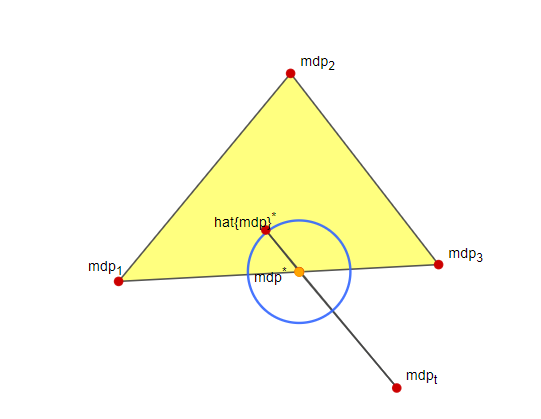
\includegraphics[width=0.45\textwidth]{img/bound}
    \caption{Model space geometry of the bound discussed in this section. The target MDP $\mdp_t$ is non-realisable and the best approximation in the realisable set is $\mdp^{*}$. The ML-estimator estimating $\mdp^{*}$ gives us a set of plausible models, constrained by the convex set. The model furthest away from the target model is $\hat{\mdp}^{*}$.}
\end{figure}

Even-Dar~\cite{even2009online} could possibly be the citation for this bound.

\begin{align}
    &||\mdp_1-\mdp_2||_1 \leq \delta \leq D_{KL}(\mdp_1 || \mdp_2)\\&\implies ||V_{\mdp_1}^\pol-V_{\mdp_2}^\pol||_\infty \leq \frac{\epsilon}{(1-\gamma)^2}
\end{align}

\hecomment{It's possible we can also say something about the stability in the linear case if the spectral radius is bounded.}

Lemmas of interest:

Mixing, $d, d'$ are distributions of states, $P^\pol$ the transition model given policy $\pol$. $\tau$ mixing time.
\begin{equation}
    ||d P^\pol - d' P^\pol||_1 \leq e^{-1/\tau}||d-d'||_1
\end{equation}

State distribution,
\begin{equation}
    ||d_{\pol, t}-d_\pol||_1 \leq 2e^{-t/\tau}
\end{equation}

Value function,
\begin{equation}
    Q_{\pol, r}(s, a) \leq 3\tau
\end{equation}

\subsection{Value Estimation Error}

The value estimation error arises when trying to estimate $V^{*}_{\mdp_t}$ given that we actually know the model $\mdp_t$. This bound, for discrete MDPs, should be available to get as a finite sample bound for \textsc{ValueIteration}.

\subsection{Model Estimation Error}

The second part of the error terms involve correctly estimating the maximum likelihood-model $\mdp^{*}$ from data $\mathcal{D}_t$.

\subsection{Realizability Error}

The third and final part of the error term is related to the difference between the best possible model in the convex set $\mathcal{C}(\mathcal{M}_s)$ and the actual target MDP $\mdp_t$. Since we have a bound on the difference in MDP $KL(\mdp_t \, || \, \frac{1}{N}\sum_{\mdp \in \mathcal{M}_s} \mdp) \leq \delta$, we should be able to get a bound also on the value function here.

\iffalse
\section{Stability of TRLOC}\label{sec:stability}

We know that systems can be stable under control input given some properties. Now what if we have a controller policy for one system, and we know that that system is very close to another system, what can we say about stability in that system under the first's controller?

\begin{definition}{Lyapunov Stability}
    A time-discrete linear system $\bm{x}_{t+1} = \mathbf{A}\bm{x}_t$ is asymptotically stable if all the eigenvalues of a $\mathbf{A}$ are less than 1.
\end{definition}

\begin{lemma}{(LQR Stability~\cite{gravell2019learning})}
    A gain $K$ is stabilising if and only if the spectral radius $\rho(\mathcal{F}_K) < 1$.
\end{lemma}

The stability implies $\underset{t\rightarrow\infty}{\lim} \mathbb{E}[\bm{x}_t\bm{x}_t^\top] = 0$, which occurs when $\theta_\Sigma$ is finite.
\fi

\section{Experiments}\label{sec:experiments}

\subsection{Discrete MDPs}

We evaluate our algorithms for discrete MDPs and settings of \emph{Type I-VI}. We assume the reward functions are identical, and put our interest into MDPs with different transition matrices. We evaluate our algorithms against a benchmark that simply uses \emph{PSRL} with the data from the target MDP to show that knowledge transfer from the source MDPs help with performance.

The algorithms we are evaluating are thus, \emph{PSRL}, \emph{EM-MMBI}, \emph{EM-PG} and possibly a fully Bayesian algorithm that does model selection correctly.

% \begin{figure}[h!]
%     \centering
%     \includegraphics[width=0.45\textwidth]{img/likelihood_experiment}
%     \caption{Likelihood experiment with $100$ independent runs. The number of models considered was $10$. The thick blue line is the mean likelihood for the true model $\mdp_t$ averaged over experiments.}
% \end{figure}

% \begin{figure}[h!]
%     \centering
%     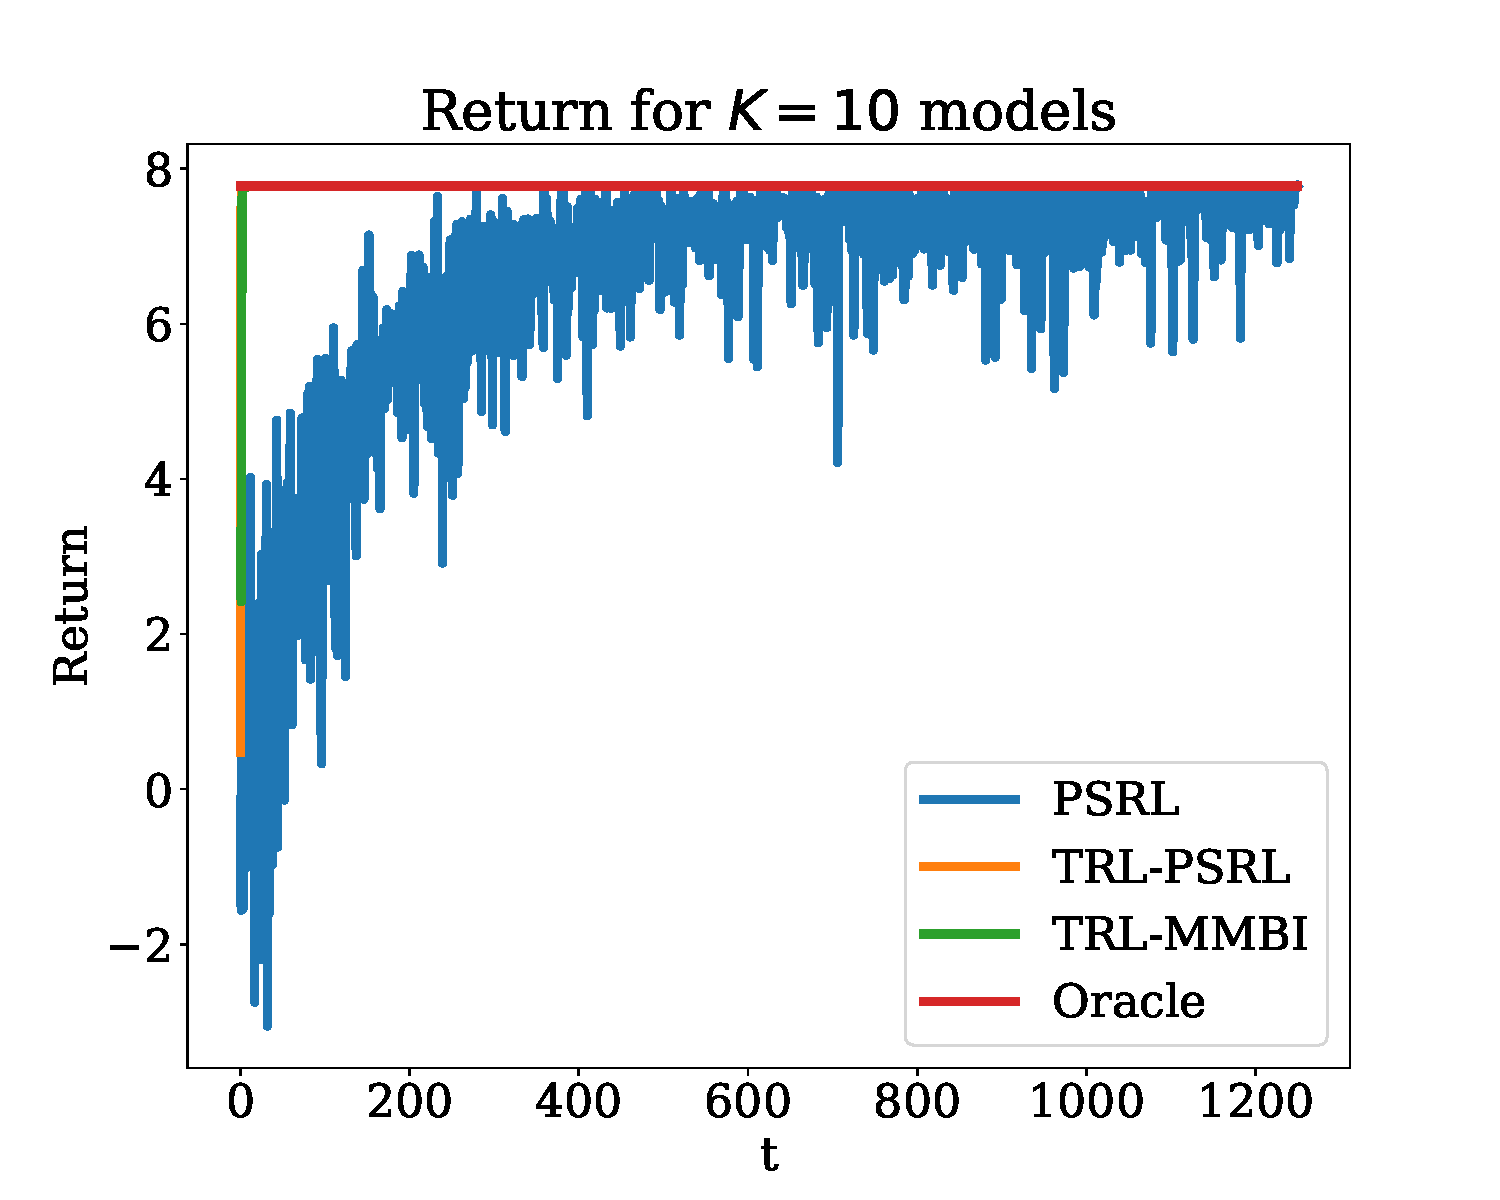
\includegraphics[width=0.45\textwidth]{img/type_I}
%     \caption{Experiment of type I. The oracle agent knows which MDP generates the data $\mathcal{D}_t$. The TRL-MMBI agent uses the likelihood $\Pr(\mathcal{D}_t \, | \, \mdp)$ to weigh the MDPs. PSRL learns the MDP from scratch using $\mathcal{D}_t.$}
% \end{figure}

% \begin{figure}[h!]
%     \centering
%     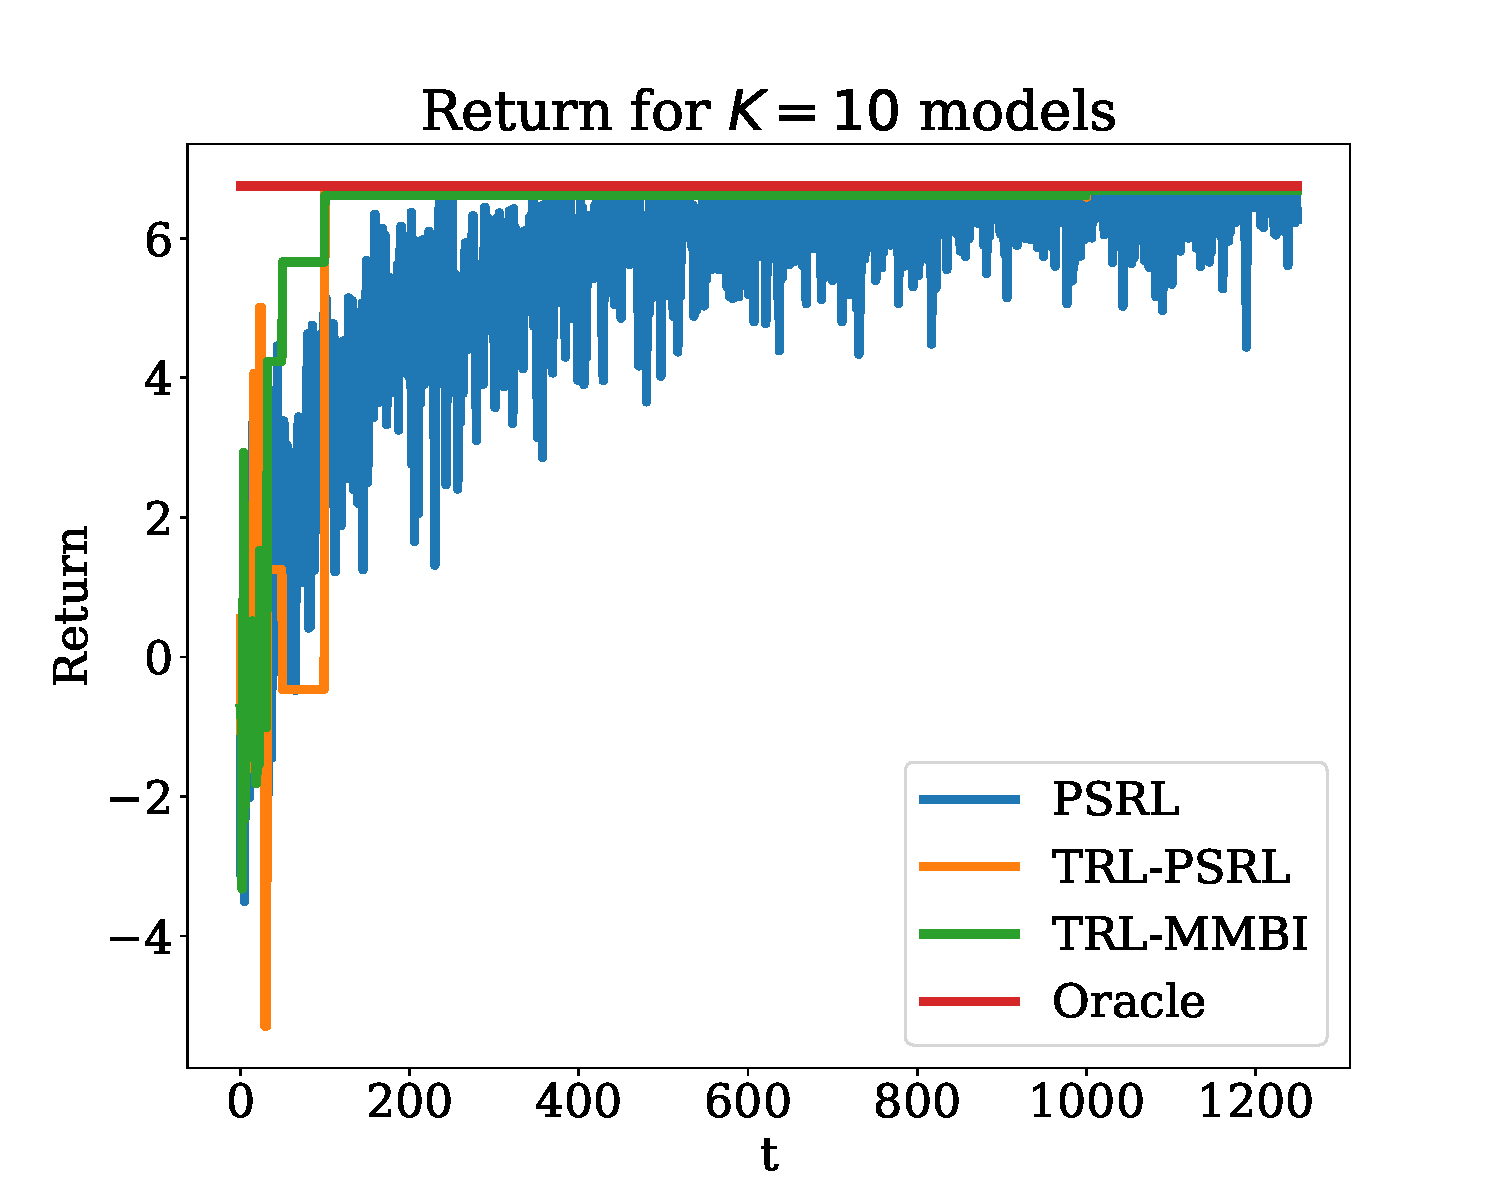
\includegraphics[width=0.45\textwidth]{img/type_II}
%     \caption{Experiment of type II. The oracle agent knows which MDP generates the data $\mathcal{D}_t$. The TRL-MMBI agent uses the likelihood $\Pr(\mathcal{D}_t \, | \, \mathcal{D}_i, \mdp)$ to weigh the MDPs. PSRL learns the MDP from scratch using $\mathcal{D}_t.$}
% \end{figure}

% \begin{figure}[h!]
%     \centering
%     \includegraphics[width=0.45\textwidth]{img/convergence_type_III}
%     \caption{Experiment of type III. Testing convergence of the minimiser using SLSQP to find the point in the simplex that corresponds to the convex MDP with the lowest negative log-likelihood. The MDP $\mdp^{*} = \sum_{i=0}^K w_i \mdp_i$ is the corresponding MDP the minimiser converged to. $\mdp^{Oracle} = \sum_{i=0}^K w_i^{Oracle} \mdp_i$ is the MDP that corresponds to the MDP in the convex set at a given point in the simplex. The data $\mathcal{D}_t \sim \mdp^{Oracle}$.}
% \end{figure}

% \begin{figure}[h!]
%     \centering
%     \includegraphics[width=0.45\textwidth]{img/optimization_type_III}
%     \caption{Experiment of type III.}
% \end{figure}

% \begin{figure}[h!]
%     \centering
%     \includegraphics[width=0.45\textwidth]{img/convergence_type_II}
%     \includegraphics[width=0.45\textwidth]{img/convergence_type_III}
%     \caption{Experiment of convex MDP. The left plot is made using PCA over the model space.}
% \end{figure}

% \hecomment{TODO: make interesting gridworld AD scenario}

\subsection{Continous Space and Action}

Further we evaluate our algorithms in continuous state and action spaces. For instance, CartPole, Mujoco.

\begin{table*}[t]
    \centering
    \begin{tabular}{c c c c c c c c}
    & & & $\mdp_t \in \Delta$& & &$\mdp_t \notin \Delta$ &\\
        Environment & Type & $\alpha=0$ & $\alpha=1$ & $\alpha=2$ & $\alpha=3$ & $\alpha=4$ & $\alpha=5$ \\ \hline
          \emph{CartPole} & I & & & & & & \\
          & III & & & & & & \\
          \emph{dm\_LQR\_2\_1} & I & & & & &\\
           & III & & & & &\\
          \emph{dm\_LQR\_6\_2} & I & & & & & \\
           & III & & & & &\\
    \end{tabular}
\end{table*}

\begin{table}[]
    \centering
    \begin{tabular}{c c c c c}
         $200.00$& $31.63$& $38.9$& $35.87$& $37.10$ \\
         $200.00$& $200.00$& $57.91$& $61.62$& $200.00$ \\
         $44.22$& $29.96$& $200.00$& $34.19$& $35.54$ \\
         $200.00$& $200.00$& $28.24$& $200.00$& $200.00$ \\
         $200.00$& $200.00$& $25.97$& $125.80$& $200.00$
    \end{tabular}
    \caption{Utility matrix}
    \label{tab:my_label}
\end{table}

\begin{table}[]
    \centering
    \begin{tabular}{c c c c c c}
    & & & $\mdp_j$ & & \\ \\
         & $0.00$& $168.37$& $161.10$& $164.13$& $162.90$ \\
         & $0.00$& $0.00$& $142.09$& $138.38$& $0.00$ \\
         $\pi^{*}(\mdp_i)$& $155.78$& $170.04$& $0.00$& $165.81$& $164.46$ \\
         &$0.00$& $0.00$& $171.76$& $0.00$& $0.00$ \\
         &$0.00$& $0.00$& $174.03$& $74.20$& $0.00$
    \end{tabular}
    \caption{Regret matrix}
    \label{tab:my_label}
\end{table}

% \begin{figure}[h!]
%     \centering
%     \includegraphics[width=0.95\textwidth]{img/BLR-LQR-return.pdf}
%     \caption{Experiment of CartPole for PSRL over $100$ experiments. The shaded region is the the standard error of the mean over experiments.}
% \end{figure}

\section{Autonomous Driving Scenarios with Knowledge Transfer}\label{sec:ad_experiments}

Random fourier features to linear mdps

free lunch with noise \url{https://arxiv.org/pdf/2111.11485.pdf}

\subsection{Setting 1: Transfer knowledge from similar tasks, e.g. cut-in to overtake}

\hecomment{Motivation: here we transfer knowledge from one or multiple tasks to a new task, which might have similar structure to it (in the MDP)}

\subsection{Setting 2: Transfer knowledge from similar cars, e.g. sedan to combi}

\hecomment{Motivation: an optimal controller must necessarily take into account the dynamics of the Ego vehicle. If a controller is learned for a smaller car, it's unlikely it will be optimal for a heavier car.}

\subsection{Setting 3a: Transfer knowledge from similar driving locations, e.g. USA to China, using traffic rules, left-side / right-side traffic}

\hecomment{Motivation: in different countries we have different traffic rules, etc.}

\subsection{Setting 3b: Transfer knowledge from similar driving locations, e.g. USA to China, using driver interaction}

\hecomment{Motivation: likewise as the previous, in different countries we have different kinds of drivers, behaviors, etc.}




